\documentclass[a4paper, 11pt]{article}

\usepackage[utf8]{inputenc}
\usepackage[T1]{fontenc}
\usepackage[francais]{babel} 
\usepackage{amsmath} % pour les formules de maths
\usepackage{amssymb} % pour des symboles
\usepackage{mathrsfs} % pour avoir acces a des jolies lettres calligrafiées.:)
\usepackage{listings} % pour le code source
\usepackage{color} % pour les couleurs
\usepackage{graphicx} % pour les graphiques (images)
\usepackage{fancyhdr} % pour utiliser le pagestyle fancy
\usepackage[headheight=10pt]{geometry} % pour les marges
\usepackage[T1,hyphens]{url}
\usepackage{float}
\usepackage{titlesec}
\usepackage{cite}

\usepackage[perpage, bottom]{footmisc}
\usepackage[colorlinks,urlcolor=blue, linkcolor=blue]{hyperref}
\usepackage[colorlinks,urlcolor=blue, linkcolor=blue]{hyperref}


%%%%%%%%%%%%%%%%%%%%%%%%%%%
% define subsubsubsection %
%%%%%%%%%%%%%%%%%%%%%%%%%%%

\titleclass{\subsubsubsection}{straight}[\subsection]

\newcounter{subsubsubsection}[subsubsection]
\renewcommand\thesubsubsubsection{\thesubsubsection.\arabic{subsubsubsection}}
\renewcommand\theparagraph{\thesubsubsubsection.\arabic{paragraph}} % optional; useful if paragraphs are to be numbered

\titleformat{\subsubsubsection}
  {\normalfont\normalsize\bfseries}{\thesubsubsubsection}{1em}{}
\titlespacing*{\subsubsubsection}
{0pt}{3.25ex plus 1ex minus .2ex}{1.5ex plus .2ex}

\makeatletter
\renewcommand\paragraph{\@startsection{paragraph}{5}{\z@}%
  {3.25ex \@plus1ex \@minus.2ex}%
  {-1em}%
  {\normalfont\normalsize\bfseries}}
\renewcommand\subparagraph{\@startsection{subparagraph}{6}{\parindent}%
  {3.25ex \@plus1ex \@minus .2ex}%
  {-1em}%
  {\normalfont\normalsize\bfseries}}
\def\toclevel@subsubsubsection{4}
\def\toclevel@paragraph{5}
\def\toclevel@paragraph{6}
\def\l@subsubsubsection{\@dottedtocline{4}{7em}{4em}}
\def\l@paragraph{\@dottedtocline{5}{10em}{5em}}
\def\l@subparagraph{\@dottedtocline{6}{14em}{6em}}
\makeatother

\setcounter{secnumdepth}{4}
\setcounter{tocdepth}{4}

%%%%%%%%%%%%%%%%%%%%%%%%
% end subsubsubsection %
%%%%%%%%%%%%%%%%%%%%%%%%


\geometry{hmargin=3cm}

\title{Projet de Master}
\author{Romain Mencattini}
\date{\today}

\pagestyle{fancy} % pour avoir des entetes et des pieds de page
\renewcommand\headrulewidth{0.6pt}
\fancyhead[L]{Romain Mencattini} % haut de page gauche
\fancyhead[R]{Université de Genève \today} % haut de page droite

\begin{document}
\maketitle
\newpage
\tableofcontents
\newpage

%%%%%%%%%%%%%%%%%%%%%%%%%%%%%%%%%%%%%%%%%%%%%%%%%%%%%%%%%%%%%%%%%%%%%%%%%%
% début l'introduction     %%%%%%%%%%%%%%%%%%%%%%%%%%%%%%%%%%%%%%%%%%%%%%%
%%%%%%%%%%%%%%%%%%%%%%%%%%%%%%%%%%%%%%%%%%%%%%%%%%%%%%%%%%%%%%%%%%%%%%%%%%
\section{Introduction}

\paragraph{}
Le but de ce projet est d'utiliser des techniques de \textit{machine learning} dans le cadre de la finance. Plus précisément, 
nous allons reprendre des techniques algorithmiques pour créer un programme de \textit{trading} de taux de changes.

\paragraph{}
Nous allons dans un premier temps faire un état de l'art. Ce dernier sera composé de
plusieurs parties.

La première traitera la marché des taux de changes afin d'obtenir les connaissances pour comprendre les enjeux et les buts recherchés.
Il s'agira d'une introduction d'éléments de bases mais néanmoins essentiels à la compréhension des algorithmes.

La deuxième partie plus mathématique abordera l'aspect théorique de plusieurs algorithmes clefs.
Soit :
\begin{itemize}
\item Les réseaux de neurones.
\item Les arbres de décision.
\item Les algorithmes \textit{SVM}.
\item \textit{Logistic Regression}.
\item \textit{Naive Bayes}.
\item Descente du Gradient.
\end{itemize}

\paragraph{}
Ensuite, nous verrons l'application de la théorie à notre cas concret, le marché des change; leurs problèmes, limitations et
solutions rencontrés ainsi que les résultats concernant les performances des programmes.

Pour conclure, nous justifierons le choix de l'algorithme ainsi que les éléments clefs du \textit{machine learning}.

\paragraph{}
Après l'état de l'art, nous implémenterons l'algorithme ou une analyse plus poussée de sa partie mathématique sera effectuée,
mais également de son application au domaine financier. Nous analyserons également les problèmes et solutions rencontrés.

Une fois l'implémentation terminée, plusieurs \textit{benchmark} seront effectués afin d'estimer les améliorations les plus
pertinentes et la performance générale de l'algorithme.

\paragraph{}
Finalement, nous analyserons les résultats et déduirons des conclusions. De plus une analyse de la pertinence de l'algorithme et des
optimisations sera réalisée et nous proposerons des pistes d'améliorations.


%%%%%%%%%%%%%%%%%%%%%%%%%%%%%%%%%%%%%%%%%%%%%%%%%%%%%%%%%%%%%%%%%%%%%%%%%%
% début de l'état de l'art %%%%%%%%%%%%%%%%%%%%%%%%%%%%%%%%%%%%%%%%%%%%%%%
%%%%%%%%%%%%%%%%%%%%%%%%%%%%%%%%%%%%%%%%%%%%%%%%%%%%%%%%%%%%%%%%%%%%%%%%%%
\section{État de l'art}
\subsection{Introduction}
\paragraph{}
Avant la démocratisation de l'informatique, les opérations financières étaient réalisées par des humains. 
Ce système pouvait avoir des inconvénients:
\begin{itemize}
\item L'émotionnel influençait les transactions. En effet, ces dernières étant effectuées par des humains, 
il y avait un risque non négligeable que l'état de la personne agisse sur sa décision.

\item Un problème sous-jacent était de maintenir une discipline de \textit{trading}. 
Afin de minimiser les pertes et de maximiser les gains, il fallait se tenir à un plan afin de ne pas se laisser 
influencer par des paramètres extérieurs. Cela pouvait être très difficile.

\item Le \textit{backtesting}\footnote{Le \textit{Backtesting} est le processus qui consiste à tester une stratégie
de \textit{trading} sur des données historiques afin de s'assurer de sa viabilité avant de risquer du capital.
\cite{investopedia_backtesting}} 
était impossible. Tester la qualification ainsi que la qualité de \textit{trading} d'une personne était compliquée. 
De même pour un \textit{trading plan}.
\end{itemize}

\paragraph{}
Ces éléments ont, en partie, favorisé l'émergence et l'utilisation d'algorithmes dans la finance. 
En 2014 aux États-Unis, 84\% des transactions étaient accomplies par des algorithmes \cite{real_investors}. 
Ce qui représente environ 100'000 réalisations, ou \textit{ticks}, par secondes \cite{real_investors}.
Durant l'évolution de l'outil informatique, le monde de la finance en a suivi les améliorations afin de perfectionner 
leurs algorithmes. On retrouve donc des méthodes d'optimisations poussées ainsi que les récentes découvertes 
de \textit{data mining} et de \textit{machine learning}, abrégé \textit{ML}. 
Des propositions de plus en plus pointues dans les deux domaines voient le jour. 
L'algorithme qui sera au coeur de ce projet en fait partie. 
Il s'agit d'un réseau de neurones avec plusieurs couches prenant en compte des paramètres particuliers à la finance.

\paragraph{}Afin d'approcher aux mieux ces notions, nous allons discuter des éléments nécessaires à leur compréhension.
Nous allons en premier lieu traiter le domaine financier ainsi que ces outils. Puis nous parlerons de 
plusieurs méthodes de \textit{ML}.
Voici celles vont être développées dans cet état de l'art:
\begin{itemize}
\item Les réseaux de neurones.
\item Les arbres de décision.
\item Les algorithmes \textit{SVM} \cite{wikipedia_svm}.
\item \textit{Logistic Regression}.
\item \textit{Naive Bayes}.
\item Descente du Gradient \cite{wikipedia_descente_du_gradient} ainsi que sa version dite stochastique \cite{descente_du_gradient_stochastique}.
\end{itemize}

Finalement, nous lierons les deux domaines en montrant comment adapter les modèles mathématiques de \textit{ML} pour les utiliser comme techniques de \textit{trading}, en évaluant leur performances.


\subsection{Finance}

\subsubsection{\textit{FOREX}}

\paragraph{}Afin d'appréhender le fonctionnement du \textit{FOREX}, il est important de mentionner certaines décisions historiques. Ces dernières ayant façonné le marché des devises actuel.

\paragraph{}
Jusqu'à la première guerre mondiale, le système en vigueur se basait sur l'or, que l'on nommait l'étalon-or\footnote{Source: \cite{etalon_or_a_etalon_dollar}.}. S'en suit une période d'instabilité notamment dûe aux pertes occasionnées par la guerre, un après-guerre compliqué, la crise boursière de 1929 et la seconde guerre mondiale.

C'est au sortir de cette dernière, que la nécessité de "\textit{mettre en place une organisation monétaire mondiale et de favoriser la reconstruction et le développement économique des pays touchés par la guerre}" \cite{wikipedia_bretten_woods}, est apparue. Le but était également "\textit{d’aplanir les conflits économiques, reconnaissant par là les problèmes engendrés par les disparités économiques}" \cite{etalon_or_a_etalon_dollar}.

Plusieurs idées furent proposées, mais ce fût celle de Harry Dexter White qui fût mise en place. Cette dernière prévoyait entre autre:
\begin{itemize}
\item le choix du Dollar américain comme étalon, avec rattachement à l'or\footnote{Suspension de l'équivalence or pour le dollar américain en août 1971 puis abandon définitif en mars 1973 \cite{wikipedia_bretten_woods}.}.
\item Création de la Banque internationale pour la reconstruction et le développement (BIRD) qui deviendra la banque mondiale.
\item Le Fond monétaire international (FMI).
\item Création de l'Organisation mondiale du commerce\footnote{Ne verra le jour qu'en 1995 faute d'accord \cite{wikipedia_bretten_woods}.}.
\end{itemize}

On remarque que ces institutions sont toujours en activités, 
cela démontre l'importance de ces accords pour le système financier actuel.

\paragraph{}
Le marché \textit{FOREX} porte sur les devises. La valeur d'une devise ne peut être exprimée qu'en fonction d'une autre. 
Par exemple 1 franc suisse vaut 1.05 euro.\footnote{Taux fictif utilisé pour l'exemple.}
La transaction porte donc sur deux monnaies comme CHF/EUR. On va vendre des francs suisses pour acheter des euros ou l'inverse.
Le nom du marché vient d'ailleurs de ces échanges. 
On échange une monnaie contre une autre, c'est un \textit{FOreign EXchange}, ou \textit{FOREX}.

Il y a deux variations possibles:
\begin{itemize}
\item La monnaie peut subir une dépréciation.
\item La monnaie peut subir une appréciation.
\end{itemize}
Lorsque le prix d'une devise augmente par rapport à une monnaie étrangère, on parle d'appréciation. 
Ainsi dans le cas contraire, on parlera d'une dépréciation.

La mondialisation a facilité ce marché. En effet, toutes devises étant accessibles depuis 
n'importe où, il devient donc possible d'avoir des marchés avec des devises plus exotiques.

\paragraph{}
Les principaux acteurs financiers sont \cite{marche_des_changes}:
\begin{itemize}
\item Les banques commerciales. 
Elles peuvent pratiquer des interventions directes car elles gèrent des dépôts et veulent opérer des transactions sur ces derniers.
Il leur est également possible de réaliser le rôle d'intermédiaire financier.

\item Les entreprises. Ces dernières vont pratiquer des transactions directes, si elles disposent d'un accès aux marchés
sinon via des intermédiaires.

\item Les institutions financières non-bancaires. On peut citer les fonds de pensions, les sociétés d'assurances
ou les \textit{hedge funds}. Ce sont surtout dans un but de spéculation, d'arbitrage ou de couverture de risque qu'elles agissent.

\item Les banques centrales. Il peut y avoir des interventions directes, dans le but de modifier l'appréciation de la monnaie.

\item Les ménages. Surtout dans une optique de voyage, d'achat ou de spéculation.
\end{itemize}

\paragraph{}
Henry Bourguinat a énoncé "\textit{la règle des trois unités}" qui correspondent aux unités de temps, de lieu 
et d'opérations et d'acteurs.
Le \textit{FOREX} répond à ces trois unités \cite{site_fr_forex}:
\begin{itemize}
\item Ce marché fonctionne 24h/24 et les transactions s'effectuent presque en continue.

\item Il fonctionne à l'échelle mondiale tout en étant décentralisé. 
De part l'évolution des technologies, l'information circule aisément malgré son statut.

\item L'uniformité des procédés ainsi que des produits est présente. Les acteurs malgré nationalité sont de même nature.
\end{itemize}

\paragraph{}
Il existe principalement deux horizons temporels: le \textit{spot} et le \textit{forward}.

Le premier est également appelé "Le marché au comptant". Lorsque deux acteurs se mettent d'accord sur une transaction,
cette dernière se réalise 
immédiatement\footnote{Valable en théorie, dans la réalité cela peut prendre du temps \cite{marche_des_changes}}.

Le second peut être nommé "Le marché à terme". L'accord est passé à un temps $T$ mais la transaction effective ne
se réalise que dans le futur. Ce futur, ou maturité, peut être de plusieurs dizaines de jours,
voir des années, soit $T + X$\footnote{Où $T$ est le moment présent, et $X$ une durée de temps.}.

Il y a des opérations réalisable sur le marché à terme.:
\begin{itemize}
\item Les \textit{swaps}. Ils consistent à vendre une monnaie au comptant puis à la racheter à terme\footnote{Soit à $T+X$}.

\item Les \textit{futures/forwards}. La différence entre ces deux tient surtout à leur standardisation et leur mise en place.
Cependant le principe reste le même: on réalise une opération (d'achat ou de vente) qui ne s'effectuera qu'à maturité.

\item Les \textit{options}. Cela représente un contrat vendu par un parti (\textit{the option writer}) 
à un autre parti (\textit{the option holder}). Ce contrat offre le droit, et non l'obligation contrairement 
aux \textit{futures/forwards}, d'acheter (\textit{call}) ou de vendre (\textit{put}). Ici encore, il faut attendre la maturité
\footnote{Cela est vrai pour les options dites européennes\cite{investopedia_option_europeenne}. 
Dans le cas des options américaines\cite{investopedia_option_americaine}, le droit peut s'exercer à n'importe quel moment, offrant
ainsi une plus grande flexibilité.}.
\end{itemize}

Les options sont très versatiles. Elles peuvent être utilisées afin de spéculer ou de diminuer le risque. Voici les différents types possibles:
\begin{itemize}
\item \textbf{long call} $\rightarrow$ on achète le droit d'acheter le sous-jacent à un certain prix.
\item \textbf{short call} $\rightarrow$ on vend le droit d'acheter le sous-jacent à un certain prix.
\item \textbf{long put} $\rightarrow$ on achète le droit de vendre le sous-jacent à un certain prix.
\item \textbf{short put} $\rightarrow$ on vend le droit de vendre le sous-jacent à un certain prix.
\end{itemize}

\paragraph{}
Le \textit{bid} est le prix maximum qu'un acheteur est d'accord de payer pour un sous-jacent.
De la même manière, le \textit{ask} est le prix minimum qu'un vendeur accepte pour vendre 
un sous-jacent \cite{investopedia_bid_ask}.

La différence entre le \textit{bid} et le \textit{ask}, appelée le \textit{spread}, représente la liquidité d'un actif. 
Il est également utilisé comme marge par les \textit{broker}\cite{wikipedia_broker} et autres plateformes.



\subsection{Cadre théorique des algorithmes de \textit{Machine Learning}}
\subsubsection{Introduction}
\paragraph{}
T. Mitchell a donné une définition formelle \cite{mitchell}:
\begin{center}
"\textit{A computer program is said to learn from experience $E$ with respect to some class of tasks $T$ and
performance measure $P$ is its performance at tasks in $T$, as measured by $P$, improves with experience $E$}"
\end{center}

On a donc une tâche $T$ à accomplir, où $T$ peut consister à trier des images ou à reconnaître des motifs.
La mesure de la réussite de cette tâche $T$ est nommée $P$. C'est-à-dire la qualité du résultat du programme pour 
la tâche donnée, $T$. Si le programme améliore son résultat $P$ pour la tâche $T$ grâce à l'expérience $E$. 
Il s'agit d'un programme de \textit{machine learning}. L'expérience peut être vue comme une phase d'entraînement
ou comme le fait de retenir les réponses après avoir accompli la tâche.

\paragraph{}
Il existe deux catégories d'apprentissage:
\begin{itemize}
\item L'apprentissage supervisé.
\item L'apprentissage non-supervisé.
\end{itemize}

Dans le cas du premier, on fournit au programme, un ensemble d'entraînement\footnote{Ou d'expérience, $E$},
qui contient des réalisations ainsi que le résultat de la classification. 
Le programme va donc pouvoir utiliser ce savoir afin d'améliorer sa performance $P$.
Nous disposons donc de nombreux couples $(x_i, y_i)$ et le but est de trouver une fonction $f \in F$ telle que: $f(x) = y$.

Pour l'apprentissage non-supervisé, on fournit des données, mais sans le résultat voulu.
C'est uniquement après avoir décidé d'une valeur qu'on va signifier au programme si cette dernière est correcte.
On ne lui donnera jamais la valeur attendue. Il va donc utiliser uniquement les résultats précédents pour améliorer son $P$.

Par exemple, on désire reconnaître un certain type de voiture à partir d'images. Dans le cas de l'apprentissage supervisé,
nous allons fournir au programme un ensemble d'entraînement qui contient de nombreuses photos de voitures,
ainsi que la marque des dites voitures. L'algorithme va donc travailler avec ces données.

Par contre dans le cas de l'apprentissage non-supervisé, le programme ne pourra utiliser que les photos,
et après avoir retourné le résultat, nous lui dirons si c'est juste ou faux. Il mémorisera le résultat 
optimisera en conséquence ses réponses.

\paragraph{}
Concernant, l'ensemble d'entraînement, il y a des points à prendre en compte afin de minimiser les risques de sur-apprentissage\footnote{Le sur-apprentissage consiste à apprendre par coeur la tâche, plutôt que d'apprendre les principes pour réaliser la tâche.}, et de maximiser la qualité de nos données.
Pour ce faire il faut:\label{astuce ensemble d'entraînement}
\begin{itemize}
\item Représenter la population générale. Donc si le but est du traitement de la langue, 
il faut que la propension et la répartition des mots soient les mêmes que ceux de la langue.

\item Contenir des membres de chacune des classes. Pour reconnaître des chiffres, il est important de disposer de chacun 
des chiffres dans l'ensemble d'entraînement.
\item Contenir de grandes variations ainsi que du bruit. Afin d'éviter le sur-apprentissage, 
il faut de nombreux exemples différents, voir très différents, les uns des autres ainsi que 
du bruit\footnote{Comme des faux exemples.}.
\end{itemize}

\paragraph{}
Il est important de saisir comment fonctionne les algorithmes de \textit{machine learning}. 
Le but est d'utiliser des données, souvent de très hautes dimensionnalités\footnote{Cela signifie qu'elles 
sont représentées par un grand nombre d'attributs.}, dans des équations dont on pourra faire varier 
les paramètres afin de classifier au mieux. Le cœur des algorithmes de \textit{machine learning} 
consiste à optimiser les dits paramètres.

\subsubsection{\textit{Logistic Regression}} \label{section régression logistique}
\paragraph{}
Une régression en statistique consiste à analyser la relation entre une variable par rapport à un ensemble d'autres 
\cite{wikipedia_regression}. On veut estimer la probabilité conditionnelle, en se basant sur des variables et 
en utilisant une distribution logistique cumulative. Cette dernière a une forme semblable à une distribution Gaussienne, 
mais avec des queues épaisses et donc une \textit{kurtosis} plus élevée. La \textit{kurtosis} étant définie comme suit:
\begin{center}
$Kurt(X) = \frac{\mu_4}{\sigma^4}$, où $\mu_4$ est le quatrième moment centré et $\sigma^4$ la variance au carré. 
\end{center}
Le but est de modéliser: $P(Y=1 | X=x)$ comme fonction de x. Nous voulons donc savoir quelle est la probabilité que 
la classe\footnote{Dans ce cas, la classe désigne une réalisation de la variable aléatoire $Y$.} $Y$ vaille $1$ sachant que $X$ vaut $x$.

Le modèle de régression est le suivant \cite{machine_learning_automated_trading}:
\begin{center}
$log(\frac{p(x)}{1 - p(x)}) = \beta_0 + x \cdot \beta$
\end{center}
, où $\beta_0$ représente l'ordonnée à l'origine de la régression linéaire
, $\beta$ est le coefficient de régression, de même dimension que $x$, et $x$ la donnée dont on veut obtenir la classe.

En résolvant cette équation pour $p$, cela donne \cite{machine_learning_automated_trading}:
\begin{center}
$p(x|y) = \frac{1}{1 + e^{-(\beta_0 + x \cdot \beta)}}$
\end{center}

\paragraph{}
Dans le cadre de l'article: \textit{A Machine Learning Approach to Automated Trading} \cite{machine_learning_automated_trading}, 
l'auteur a implémenté deux variations de cet algorithme:
\begin{itemize}
\item \textit{Logistic regression with a ridge penalty}:
\begin{center}
$$\sum_{i=1}^N (y_i - \sum_j\beta_j x_{ij})^2 + \lambda \sum_j \beta_j^2$$
\end{center}
, où $y_i$ est la classe de notre observation, $\beta_j$ sont les coefficients de la régression logistique originale \cite{machine_learning_automated_trading} et $x_{ij}$
sont les $j$ éléments de l'observation $i$.

L'objectif est de minimiser le carré de la différence entre la classe, ou résultat, de $y_i$ et le résultat 
calculé: $\sum\limits_j\beta_j x_{ij}$. Donc en fonction de l'observation $x_i$ et des coefficient de $\beta$.
En ajoutant une pénalité, sur $\beta$, on va tenter d'éviter le sur-apprentissage.

\item \textit{Lasso logistic regression/ Lasso regularization}:
\begin{center}
$$\sum_{i=1}^N (y_i - \sum_j\beta_j x_{ij})^2 + \lambda \sum_j |\beta|$$
\end{center}
Le fonctionnement est similaire au précédent, seul change la pénalité.

\end{itemize}

\paragraph{}
Comme mentionné plus haut, l'optimisation porte sur les paramètres de l'équation. Dans le cas de la régression logistique, 
il s'agît du $\beta$. Il conviendra donc de trouver la valeur optimale pour cette variable afin de maximiser ou minimiser 
les équations ci-dessus. De manière similaire pour les autres techniques de \textit{ML}, 
les équations et les paramètres vont changer, mais  le but sera toujours d'optimiser ces éléments. 

\subsubsection{Les arbres de décision}\label{section arbre de décision}

\paragraph{}
Un arbre de décision est un arbre, dont chaque nœud représente un test sur un attribut. 
Les branches qui suivent directement le nœud sont les valeurs possibles de l'attribut. 
Les feuilles de l'arbre, quant à elles, sont la classification d'élément donné en entrée.

Il est important de disposer des attributs avant de commencer la construction de l'arbre. 
Lors de l'implémentation, nous pouvons représenter l'arbre comme une suite de \textit{if-then-else} afin 
d'améliorer la lisibilité. Dans ce cas très précis, disposer d'un langage permettant le \textit{pattern matching} est fort utile.

Cet algorithme a tendance à très facilement sur-apprendre, il convient donc de bien choisir la manière de construire 
l'arbre ainsi que l'ensemble d'entraînement pour minimiser cet effet. 

Voici un exemple d'arbre de décision\footnote{\url{http://cloudmark.github.io/images/kotlin/ID3.png}}:
\begin{figure}[h!]
\centering
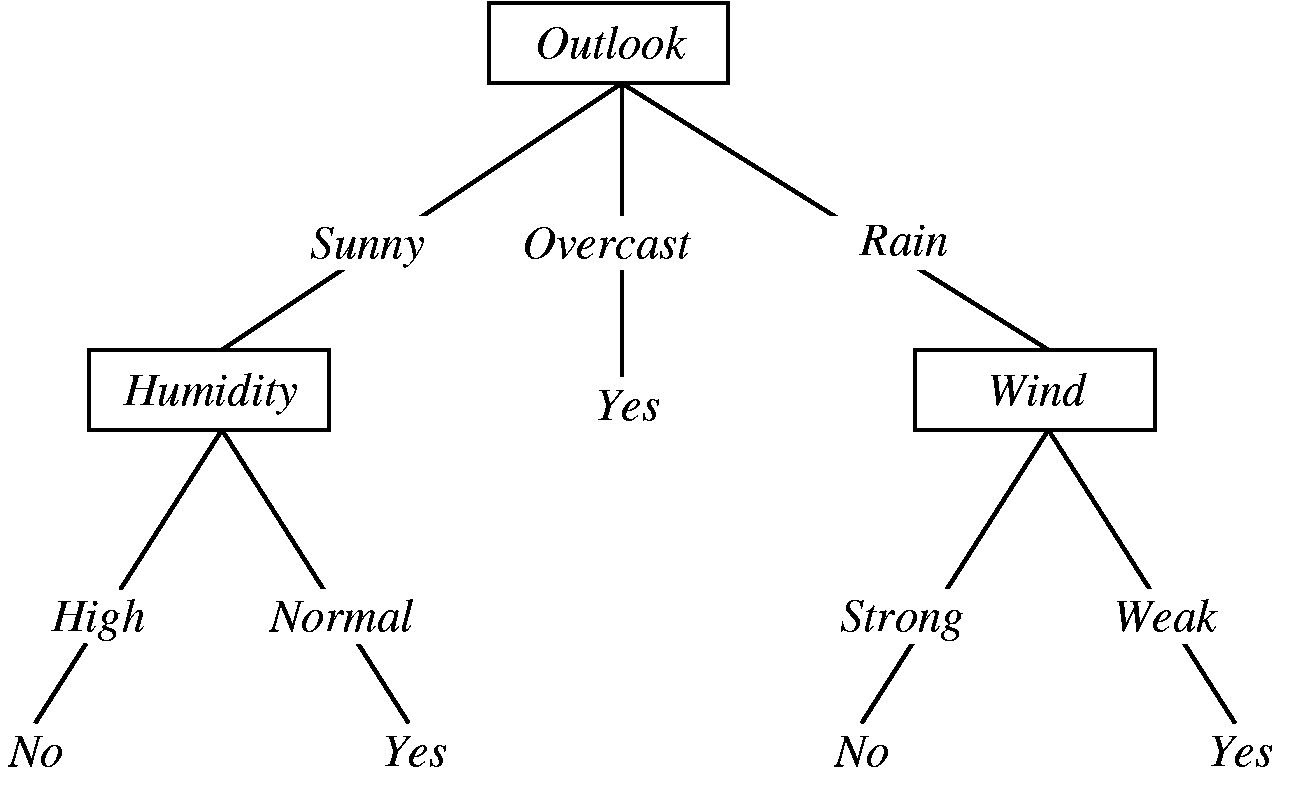
\includegraphics{images/exemple_tree}
\caption{Exemple d'arbre de décision: Permet de décider si nous pouvons aller jouer au tennis ou non.}
\end{figure}

\paragraph{}
Afin de construire l'arbre à partir de l'ensemble d'entraînement, il existe plusieurs algorithmes. 
Un des plus connus est le \textit{ID3} \cite{id3}. Il s'agit d'une méthode de type \textit{greedy}.

À chaque itération, il faut:
\begin{itemize}
 \item effectuer un test statistique\footnote{Il vise à vérifier la quantité d'information gagnée pour 
 la classification \cite{id3}.} afin de trouver l'attribut le plus discriminant.
 \item utiliser cet attribut comme nœud.
 \item retourner au premier point, tant que l'ensemble des attributs n'est pas vide.
\end{itemize}

Nous allons construire l'arbre de manière \textit{top-down} en utilisant ,à chaque pas, le meilleur attribut, selon notre test
statistique.


\subsubsection{\textit{Naive Bayes}}\label{section naive bayes}
\paragraph{}
À l'instar de la régression logistique (voir \ref{section régression logistique}), il s'agit d'un classifieur probabiliste. 
Ce dernier se base sur le théorème de Bayes\footnote{\url{https://brilliant.org/wiki/bayes-theorem/}}:
\begin{center}
$P(Y|X) = \frac{P(X|Y)}{P(X)}P(Y)$
\end{center}

À partir de cela, nous obtenons l'équation de \textit{machine learning} suivante \cite{machine_learning_automated_trading}:
\begin{center}
$V_{NB} = arg\ max_{v_{j \in V}} P(v_j) \prod\limits_i P(a_i | v_j)$
\end{center}
Où $V_{NB}$ est la classe obtenue, $P(v_j)$ la probabilité à \textit{priori} donc sans informations 
et $\prod\limits_i P(a_i | v_j)$ la probabilité de vraisemblance.
Il convient donc de trouver la classe qui maximise ce calcul.

Afin d'avoir une certaine sécurité dans les résultats, il est possible d'ajouter un seuil. 
Les réponses du classifieur étant comprise entre $0$ et $1$, le seuil permettra de décider si la réponse sera prise en compte.

Par exemple, avec un seuil de $0.6$ si $V_{NB} = 0.58$, alors la réponse n'est pas validé et le classifieur ne renvoie aucun
résultat. Si $V_{NB} = 0.7$ alors la réponse est jugée sûre et la classe de $V_{NB}$ est retournée. 

\paragraph{}\label{section roc curve analysis}
La \textit{ROC\footnote{Receiver Operating Characteristic} Curve analysis} permet d'améliorer le classifieur. 
En effet cette dernière peut détecter les \textit{true positive rate} par rapport aux \textit{false positive rate} 
pour différents seuils de classification de l'algorithme \textit{Naive Bayes} \cite{machine_learning_automated_trading}. 
À partir de cela, nous pouvons déterminer le meilleur seuil de sortie et donc perfectionner notre algorithme.
De plus cette courbe peut aider à comparer des classifieurs entre eux en comparant 
la surface sous la courbe \cite{machine_learning_automated_trading}.

La méthode utilisée est la suivante \cite{machine_learning_automated_trading}: il faut faire s'intersecter 
la pente $S$ avec la courbe \textit{ROC} et ainsi obtenir une valeur optimale pour le seuil.
Cette pente $S$ est définie comme suit \cite{machine_learning_automated_trading}:
\begin{center}
$S = \frac{Cost(P|N) - Cost(N|N)}{Cost(N|P) - Cost(P|P)} \cdot \frac{N}{P}$
\end{center}
Sachant que $Cost(P|N)$ est le coût pour avoir mal classé une classe négative comme positive. 
$P$ est la somme des vrais positifs et des faux négatifs. $N$, quant à lui, 
vaut la somme des vrais négatifs ainsi que des faux positifs.

Voici une illustration\footnote{Source: \url{http://www.prolekare.cz/dbpic/jp_5403_f_20-x1000_1600}}:
\begin{figure}[H]
\centering
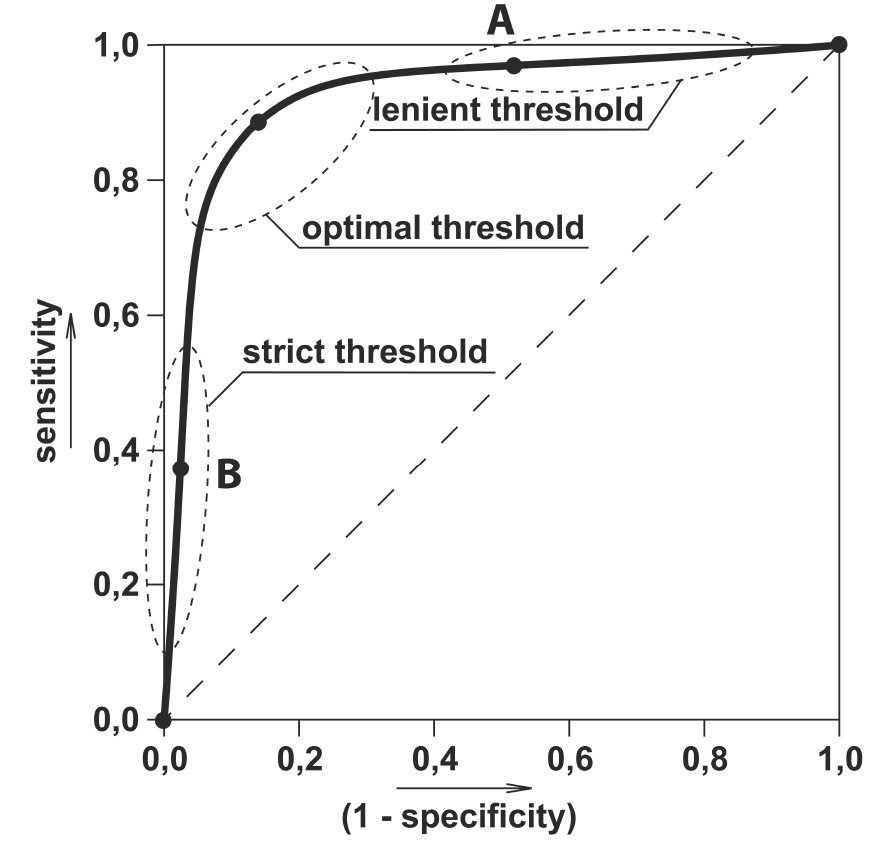
\includegraphics[scale=0.20]{images/roc_curve}
\caption{Exemple de \textit{ROC curve}: L'axe des $x$ correspond au taux de faux positifs et l'axe des $y$ 
au taux de vrais positifs. On veut donc trendre vers $y = 1$ et $x = 0$. Lors de l'optimisation par la pente $S$, 
le but sera d'obtenir une intersection avec la \textit{ROC curve} dans la zone \textit{optimal threshold} 
afin d'avoir le meilleur seuil possible.}
\end{figure}


\subsubsection{\textit{SVM}}\label{section svm}
\paragraph{}
Le but de l'algorithme \textit{SVM}\footnote{\textit{Support Vector Machine}} est de séparer les données grâce à un hyper-plan.
Cela permet de différencier les classes des observations suivantes en déterminant s'ils se trouvent d'un côté ou l'autre 
du plan. Ce dernier n'est pas unique\footnote{Source: \url{https://computersciencesource.files.wordpress.com/2010/01/svmafter.png}}: 
\begin{figure}[H]
\centering
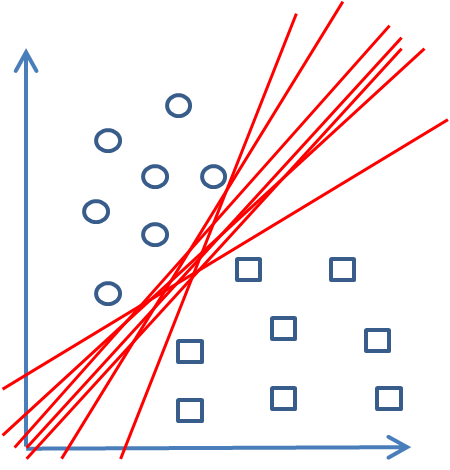
\includegraphics{images/svm_exemple}
\caption{Exemple d'hyper-plans séparant les données. Si nous voulons classifier un nouvel élément, 
il suffit de calculer s'il se trouve à gauche ou à droite de l'hyper-plan. Dans le premier cas, il s'agira, 
pour notre algorithme, d'un rond et dans l'autre d'un carré}
\end{figure}

\paragraph{}
Notre fonction est:
\begin{center}
$f(x) = (w \cdot x) + b$
\end{center}
Le but est de maximiser la distance entre les points les plus proches de l'hyper-plan, tout en pénalisant 
les points mal classés. Il n'est pas toujours possible de séparer les données de dimensions $n$, 
il conviendra donc d'augmenter la dimension afin d'obtenir une dimension $m > n$ plus discriminante. 
La fonction $\phi(x)$ est utilisée dans ce but. Un exemple de fonction est:
\begin{center}
$\phi: R^2 \rightarrow R^3 :(x, y) \rightarrow (x, y, z):= (x^2, \sqrt{2}x y, y^2)$
\end{center}

Il est possible d'imager cette opération comme cela\footnote{\url{https://www.dtreg.com/uploaded/pageimg/SvmDimensionMap.jpg}}:
\begin{figure}[H]
\centering
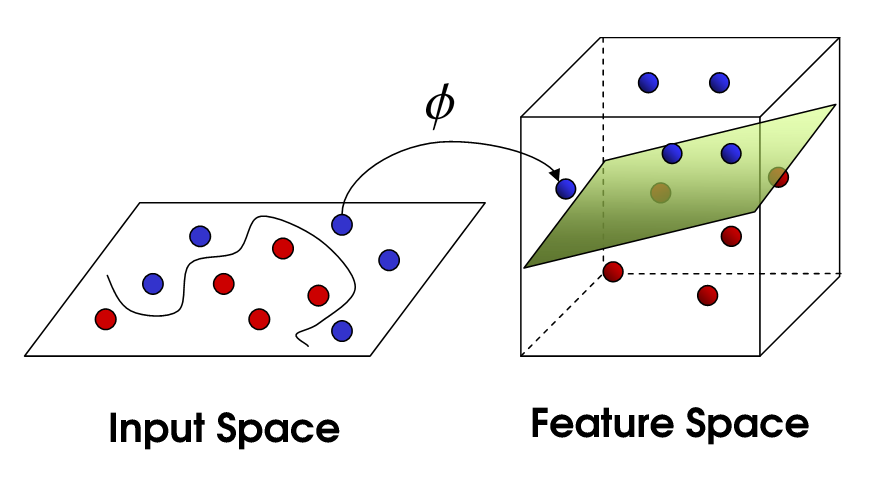
\includegraphics[scale=0.3]{images/svm_exemple_phi}
\caption{Exemple d'utilisation de la fonction $\phi$ pour passer d'un espace $R^2$ à $R^3$ afin de faciliter la séparation.}
\end{figure}


En terme d'équation, nous voulons minimiser w, dans l'équation de l'hyper-plan: $(w \cdot x) + b$. Il faut également prendre
en compte $y_i \in \{-1,+1\}$ :
\begin{center}
 \[ (w \cdot x) + b =
  \begin{cases}
    \ge +1   & \quad \text{si $y_i = +1$}\\
    \le -1 & \quad \text{si $y_i = -1$}\\
  \end{cases}
\]
\end{center}

 Ce qui donne \cite{svm_equation}:
\begin{center}
$y_i (w \cdot x_i + b) \ge 1$
\end{center}
Si malgré l'augmentation de la dimension, les données ne sont pas séparables, 
il faut tenter de minimiser le nombre d'éléments mal placés. Pour ce faire \cite{svm_equation}:
\begin{center}
$y_i (w \cdot x_i + b) \ge 1 - \xi_i$ avec $\xi_i > 0$ 
\end{center}
Afin de diminuer l'erreur et optimiser au mieux notre classifieur.


\subsubsection{Réseaux de neurones}
\paragraph{}
Tout comme les algorithmes génétiques s'inspirent de la sélection naturelle dans un but d'optimisation,
les réseaux de neurones se basent sur un modèle formel de neurones
\footnote{Neurones formels: \url{http://www.peoi.org/Courses/Coursesfr/neural/neural3.html}} afin de copier la capacité 
d'apprentissage des êtres vivants.

Il s'agit d'opérer à partir de données en entrée, des \textit{inputs}, une ou plusieurs multiplications matricielles
en utilisant des vecteurs de poids, des \textit{weights}. L'optimisation s'applique sur les \textit{weights},
afin de maximiser la classification.

Un réseau de neurones peut avoir plusieurs couches, \textit{layers}. Dans ce cas, la première couche est
appelée \textit{input layer}, la dernière \textit{output layer} et toutes celles entre ces deux sont
les \textit{hidden layers}. De plus, les neurones peuvent être pleinement connectés avec ceux de la couche
suivante, \textit{feed-forward}; ce qui signifie que les neurones de la couche $n-1$ influencent ceux de
la couche $n$. Il est également possible que les éléments de $n$ agissent sur les neurones de $n-1$, ce
phénomène est appelé \textit{feedback networks}.

\begin{figure}[H]
\centering
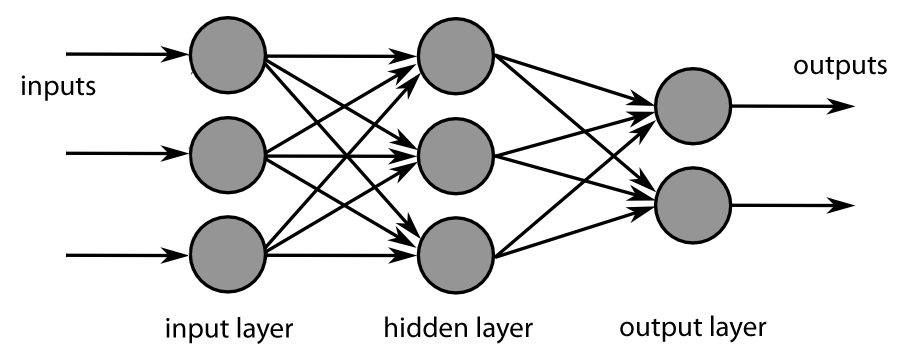
\includegraphics[scale=0.4]{images/neural_net_feedforward}
\caption[]{Exemple d'un réseau de neurones avec plusieurs couches. Illustre également
le \textit{feed-forward}: l'\textit{ouput} de l'\textit{input layer} est propagé dans chaque
neurones de l'\textit{hidden layer}. Même chose pour les deux dernières couches.\footnotemark}
\end{figure}

\begin{figure}[H]
\centering
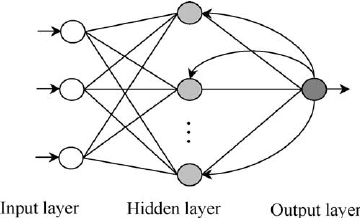
\includegraphics{images/neural_net_feedback}
\caption[]{Exemple d'un réseau de neurones avec plusieurs couches. Dans ce cas là,
les couches font du \textit{feed-forward} mais de plus, le \textit{feedback} est utilisé afin
d'influencer les couches précédant l'\textit{output layer}.\footnote[2]{}}
\end{figure}

\footnotetext{Source: \url{http://web.utk.edu/~wfeng1/spark/_images/fnn.png}}
\stepcounter{footnote}\footnotetext{Source:\url{https://jcrisch.files.wordpress.com/2015/04/reseau_de_neurones.png}}

\paragraph{}
Concernant la valeur de sortie, elle peut être simple, comme le résultat d'une classification binaire,\textit{i.e.} $0$ ou $1$
en sortie. Mais elle peut également être d'une dimensionnalité plus élevée comme un vecteur, citons l'exemple d'un point
dans un espace $R^2$.

Afin de borner les valeurs en sortie, la plupart des réseaux utilisent une fonction. Nous pouvons citer :
\begin{itemize}
\item La fonction sigmoïde : $S(t) = \frac{1}{1 + e^{-t}}$.
\item La fonction tangente hyperbolique : $f(x) = tanh(x)$.
\end{itemize}

Bien souvent, l'utilisation d'un réseau de neurones à une couche est suffisante. Cela est valable pour les fonctions continues,
dans le cas de fonctions discontinues, il est intéressant de passer à un réseau disposant de plusieurs couches.
Attention toutefois, si le nombre de neurones est trop important, l'algorithme va avoir tendance à sur-apprendre,
et à l'inverse, à sous-apprendre si le nombre est trop faible. Il est donc important de bien doser cette quantité afin
d'éviter ces problèmes.

\paragraph{}
Un exemple concret de réseau de neurones est celui présenté dans l'article qui se trouve au cœur du projet ~\cite{fx_trading}.
Avant de montrer les équations, en voici un schéma \cite{fx_trading}:
\begin{figure}[H]
 \centering
 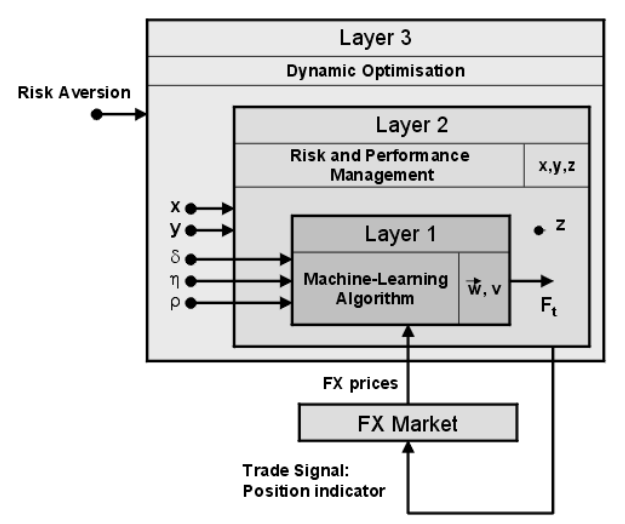
\includegraphics[scale=0.4]{images/exemple_nn_projet}
 \caption{Représentation sous forme de schéma du réseau de neurones. Avec $w$ le vecteur de poids, $v$ le seuil, $\delta$ le coût de
 \textit{trading}, $\eta$ un paramètre d'adaptation, $\rho$ le taux d'apprentissage, $x$ le seuil d'arrêt lors de pertes, $y$ le
 seuil de \textit{trading}, $z$ la condition d'arrêt automatique lors de pertes critiques et l'aversion au risque notée $\upsilon$.}
\end{figure}

Il s'agit de trois couches qui doivent optimiser chacune une série de paramètres. La première va maximiser le vecteur de poids $w$
ainsi que $v$ le seuil. À partir de ces paramètres, nous pouvons utiliser la formule suivante :
$$F_t = sign(\sum_{i=0}^M w_{i,t} r_{t-i} + w_{M+1,t} F_{t-1} + v_t)$$
où $r := p_t - p_{t-1}$ est le retour d'une position. $F_t$ nous permet de calculer la position à prendre au temps $t$ en tenant
compte de l'historique des prix.

L'optimisation de $w$ se fait par un algorithme de descente du gradient (voir \ref{section descente du gradient}).

\paragraph{}
La deuxième couche va travailler à partir des paramètres $x,y,z$. Il est possible que le marché soit irrationnel durant une longue
durée, dans ce cas la psychologie peut pousser à garder une position en espérant un changement. C'est ce genre de comportement qu'un
algorithme permet d'éviter. Pour ce faire, nous définissons un excédant des pertes et nous veillons qu'il soit toujours à une distance
$x$ du meilleur prix atteint; afin d'éviter de tenir trop longtemps une position défavorable.

Il est également intéressant de définir un seuil. Si la réponse du réseau est supérieure à ce seuil, nous la prenons en compte et
dans le cas contraire, nous ne faisons rien. Cela permet d'évaluer la "force" du signal renvoyé par la première couche. Ce seuil
est $y$.

La dernière variable utilisée dans cette couche est $z$. Il y a un consensus dans la communauté de \textit{trading} concernant le fait
que les algorithmes fonctionnent bien durant un temps puis cesse d'être profitable. À ce moment, il convient d'arrêter le programme
et d'y apporter des modifications\footnote{Au niveau des équations, des données ou des paramètres.} avant de le relancer. La tâche du
paramètre $z$ est de donner un seuil pour les pertes du profit cumulé qui, lorsqu'il est dépassé, lance une procédure d'arrêt.
Contrairement à $x,y$ qui seront optimisés par la troisième couche, le paramètre $z$ est fixé au début du programme et ne change plus.

\paragraph{}
La couche d'optimisation dynamique est la troisième couche. Cette dernière va, à chaque itération, optimiser les paramètres suivants :
$x,y,\eta,\delta,\rho$.

Pour ce faire elle va utiliser \cite{fx_trading}:
$$\Sigma := \frac{\sum_{i=0}^N (R_i)^2 I(R_i < 0)}{\sum_{i=0}^N (R_i)^2 I(R_i > 0)}$$
$$ U(\overline{R},\Sigma,\upsilon) := a\cdot(1-\upsilon)\cdot \overline{R} - \upsilon \cdot \Sigma$$

,où $R_i := W_i - W{i-1}$ est le retour au temps $i$ avec $W_i$ le profit cumulé, $\overline{R} := \frac{W_N}{N}$ est le profit moyen
avec $N$ qui est le nombre d'intervalle, $a$ une constante et $\upsilon$ l'aversion au risque.

Ces équations ont été construites de manière à posséder ces propriétés \cite{fx_trading}:
\begin{itemize}
 \item Une stratégie négative implique un risque très élevé afin d'éviter de soudaines et importantes pertes.
 
 \item Avec la définition de $\Sigma$, un large total de \textit{trading} défavorable\footnote{Calculé par :
 $\sum_{i=0}^N (R_i)^2 I(R_i < 0)$.} par rapport à l'impact total des opérations favorable\footnote{Calculé par :
 $\sum_{i=0}^N (R_i)^2 I(R_i > 0)$.} conduit à un risque important même si le profit reste le même. Cela favorise un système
 qui augmente de manière monotone ses profits plutôt qu'un autre plus irrégulier.
 
 \item La mesure $\Sigma$ pénalise uniquement les stratégies négatives et pas les stratégies positives. 
\end{itemize}

La fonction à optimiser est donc :
$$\max_{\delta, \eta, \rho, x, y} U(\overline{R};\Sigma: \delta, \eta, \rho, x, y; \upsilon)$$

Car $x,y,\eta,\delta,\rho$ interviennent tous dans le calcul de $\Sigma$. Ces derniers peuvent être optimisés de la manière voulue.
L'article ne creuse pas cette fois et utilise une recherche aléatoire composante par composante.

\subsubsection{Descente du gradient}\label{section descente du gradient}
\paragraph{}
L'algorithme de descente du gradient fonctionne sur des fonctions réelles différentiables sur un espace tel
que $\mathbb{R}^n$. Il est itératif et fonctionne donc en améliorant l'itération précédente, jusqu'à
atteindre une condition d'arrêt.

Avant d'en expliquer la teneur mathématique, voici un exemple de l'algorithme dans $\mathbb{R}^2$ :

\begin{figure}[H]
\centering
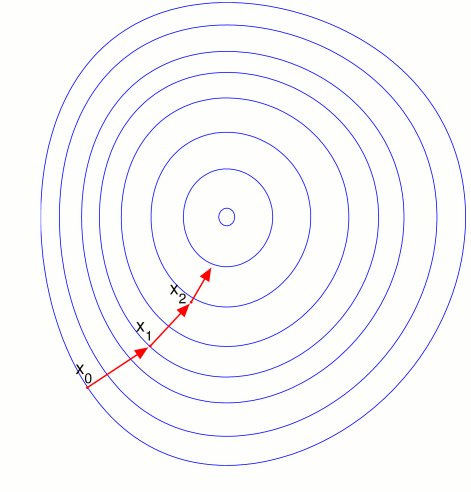
\includegraphics[scale=0.40]{images/descente_gradient_exemple}
\caption[]{Exemple de l'algorithme de descente du gradient en deux dimensions. À chaque itération,
il faut prendre la direction opposée au gradient\footnotemark, cela permet d'arriver à un nouveau
point. En itérant, on se rapproche de l'optimum. }
\end{figure}

\footnotetext{Dans cet exemple, il est possible de dire, qu'il faut prendre la normal de la courbe de niveau.}

\paragraph{}
Afin de comprendre, les divers algorithmes, il est important d'avoir les connaissances mathématiques
sur ce sujet. L'algorithme se définit comme suit\footnote{Inspiré de \cite{wikipedia_descente_du_gradient}.}:

\paragraph{}
Soit un point initial $x_0 \in \mathbb{R}$. Soit $\epsilon > 0$ un seuil de tolérance. L'algorithme définit
une suite d'itération $x_1,x_2,.. \in \mathbb{R}^n$, jusqu'à ce qu'un test d'arrêt soit satisfait.
Pour passer de $x_i$ à $x_{i+1}$, il faut :
\begin{itemize}
\item Calculer $\bigtriangledown f(x_k)$

\item Si $||\bigtriangledown f(x_k)|| \le \epsilon$ alors arrêt.

\item Sinon il faut calculer $\alpha_k$ par recherche linéaire\footnote{La recherche linéaire consiste à choisir une direction
 de descente afin de minimiser une fonction donnée jusqu'à atteindre l'optimum ou un seuil fixé 
\cite{wikipedia_recherche_lineaire}.} sur $f$ en $x_k$. Cette recherche se fait dans la direction opposée au gradient,
soit $-\bigtriangledown f(x_k)$. Une fois $\alpha_k$ calculé, il faut mettre à jour le
point itéré : $$x_{k+1} = x_k - \alpha_k \bigtriangledown f(x_k)$$
\end{itemize}

\paragraph{}
La preuve que la recherche dans la direction opposée au gradient induit une décroissance est la suivante.
Si la dérivée est non nulle\footnote{i.e: Si nous ne sommes pas déjà sur un maximum} au point $x$, $f'(x) \ne 0$. Soit
$$d = - \bigtriangledown f(x)$$
Puisque :
$$f'(x) \cdot d = \bigtriangledown f(x) \cdot -\bigtriangledown f(x) = - ||\bigtriangledown f(x) ||^2 < 0$$

L'égalité est strictement plus petite car la dérivée est non nulle par hypothèse. Cela implique que :
$$f(x -\alpha \bigtriangledown f(x)) < f(x)\text{,\ } \forall \alpha > 0$$

Nous avons donc que pour chaque itération, la valeur obtenue va décroître jusqu'à attendre un maximum ou le seuil $\epsilon$.

\paragraph{}
La descente du gradient d'un point de vue mathématique peut également être utilisée conjointement à un réseau de neurones. 
En effet dans cet article ~\cite{fx_trading}, les poids $w$ de la première couche, sont optimisés suivant cette formule :
$$w_{i,t} = w_{i-1,t} + \rho \bigtriangleup w_{i,t}$$

Où $t$ correspond au temps, $i-1$ à l'itération courante et $\rho$ le taux d'apprentissage.

De part la convergence de $w_i$ vers son optimum, cela permet, une fois cette valeur obtenue, de l'injecter
comme étant les poids d'un réseau de neurones.

\paragraph{}
Il existe deux types d'algorithme de descente du gradient :
\begin{itemize}
\item Le \textit{Batch Algorithm} a pour but de minimiser la fonction de coût qui aura été définie au préalable en utilisant 
toutes les données. Ce dernier peut prendre énormément de temps, de par son côté itératif, si l'ensemble d'entraînement croît.
\item Le \textit{Online Algorithm} va également minimiser une fonction de coût. Contrairement au \textit{Batch Algorithm}, il
prendra les exemples un à un. L'optimisation ne se fera que pour l'exemple courant puis recommencera sur une autre donnée. 
Cette manière de procéder s'applique aisément sur les gros volumes de données.
\end{itemize}

Provenant de cet article \cite{descente_du_gradient_stochastique}, voici des équations pouvant être minimisées dans
le cadre d'un programme de \textit{machine learning}.
Soit $(x_i,y_i)\text{,\ } i=1..N$, un ensemble de données. Notre fonction de coût est $l(y,y')$.
Cela représente le coût de prédire $y'$ quand la réponse est $y$. Moyennons cela sur tous les exemples :

$$E_N(f) = \frac{1}{N} \sum_{i=1}^{n}l(f_w(x_i),y_i)$$

Où $f_w$ est une fonction pondérée par un vecteur de poids $w$ que l'on cherche à optimiser.
Pour optimiser les poids, nous allons utiliser la descente du gradient :
$$w_{k+1} = w_k - \alpha_k \bigtriangledown f_{w_k}(x) \rightarrow w_{k+1} =
w_k -\alpha_k \sum_{i=1}^n \bigtriangledown Q ((x_i,y_i), w_k)$$

Où $Q(x,y) = l(f_w(x),y)$.

\paragraph{}
Comme mentionné plus haut, la technique de \textit{Batch Algorithm} devient lente lorsque le nombre de données augmente.
Pour pallier ce problème, il existe une technique : \textit{stochastic gradient descent}. C'est une méthode d'approximation
statistique de la descente du gradient.

Il convient de ne prendre qu'un seul couple au lieu de l'ensemble complet d'entraînement. La somme disparaît donc dans l'équation à minimiser :
$$w_{k+1} = w_k -\alpha_k \bigtriangledown Q ((x_i,y_i), w_k)$$
C'est donc une technique de \textit{Online Algorithm}. L'algorithme peut traiter des données à la volée car il n'a pas
besoin de se souvenir des exemples précédant.

Il est possible pour pénaliser la complexité de $w$ de rajouter un élément. Cela permet de borner quelque peu les valeurs des poids:
$$w_{k+1} = w_k -\alpha_k \bigtriangledown Q ((x_i,y_i), w_k) + \sigma P(w_k)$$

Où $\sigma > 0$ est un hyper-paramètre et $P$ peut valoir :
\begin{itemize}
\item \textbf{L1 norm} = $P(w) := \sum\limits_{i=1}^n |w_i|$
\item \textbf{L2 norm} = $P(w) := \frac{1}{2}\sum\limits_{i=1}^n w_i^2$
\item \textbf{Elastic Net} = $P(w) := \rho \frac{1}{2}\sum\limits_{i=1}^n w_i^2 + (1 - \rho) \sum\limits_{i=1}^n |w_i|$
\end{itemize}


\subsubsection{\textit{Majority vote}} \label{section majority vote}
\paragraph{}
Le \textit{majority vote} n'est pas strictement un algorithme de \textit{ML}. Il s'agît plutôt d'améliorer les résultats
en modifiant la manière d'utiliser certains des algorithmes pré-mentionnés.
Il est donc possible d'employer le \textit{majority vote} avec la régression logistique, les réseaux de neurones, etc.

\paragraph{}
Le principe est le suivant. Soit $E$ notre ensemble d'entraînement, soit $M = \{f_1, f_2, ...\}$ notre ensemble de
méthodes $f_i$ de \textit{machine learning}. Notons $M_E = \{f_{1_E}, f_{2_E}, ...\}$ notre ensemble de
méthodes $f_{i_E}$ entraînées.
 
\[ f_{i_E}(x) =
  \begin{cases}
    1       & \quad \text{si la classe calculée de $x$ est 1.}\\
    0  & \quad \text{si la classe calculée de $x$ est 0.}\\
    -1 & \quad \text{si aucune classe n'est trouvée ou si le seuil est insuffisant.}\\
  \end{cases}
\]

L'algorithme se comporte comme suit pour une observation $x$:
\paragraph{}
$\forall f_{i_E} \in M_E$, il faut calculer $f_{i_E}(x)$ et garder la classe résultante dans notre liste de résultat $R$.
Si $\exists\ classe_i \in R$, telle que $$\sum (classe_i \in R) > \frac{|M_E|}{2}$$

Alors cela signifie que la $classe_i$ est notre résultat, dans le cas contraire, l'algorithme ne donne aucune réponse.

\paragraph{}
L'algorithme va donc, à partir d'un ensemble de méthodes et d'une observation, calculer les classes. Si
une de ces dernières est représentée de manière majoritaire\footnote{\textit{i.e.} 50\% des voix + 1 voix}, le
programme retournera ce résultat. Si la majorité n'est pas atteinte, aucune classe n'est jugée valable et donc
aucune réponse ne sera rendue.

Cette technique réduit la composante individuelle des méthodes de \textit{ML} ainsi que le risque d'erreur. Si
une observation est mal classifiée, cela signifie que plus de la moitié des algorithmes ont fait une erreur.
Dans ce cas, il convient de changer les attributs utilisés ou l'ensemble d'entraînement car l'erreur ne
proviendra vraisemblablement pas d'un problème d'implémentation ou de la faiblesse de classification d'un algorithme particulier.

\subsubsection{\textit{Random Subset}} \label{section random subset}
\paragraph{}
À l'instar du \textit{majority vote}, le \textit{random subset} est une technique pour employer des méthodes de \textit{ML}.

\paragraph{}
Le principe est le suivant :

Il faut prendre $N$ différents ensembles de données\footnote{Il est possible de découper notre ensemble initial afin
d'atteindre ce critère.} du domaine concerné. Ils permettront d'entraîner un algorithme sur chacun d'entre
eux\footnote{Comme \textit{Naive Bayes} ou {SVM}.}. Nous disposerons donc de $N$ instances de l'algorithme de \textit{ML}
initial, mais avec un entraînement différent pour chacun, puis pour chaque observation, nous allons utiliser ces $N$ instances
afin d'obtenir un résultat de classification.

Comme pour le \textit{majority vote}, si une même classe est représentée une majorité de fois, le \textit{random subset} retournera ce résultat, et aucun le cas contraire.

\paragraph{}
Il est nécessaire d'avoir un grand jeu de données afin de fournir suffisamment d'échantillons aux instances pour qu'elles
apprennent correctement.
Une fois ce problème résolu, cette technique nous donne la possibilité d'utiliser au mieux l'ensemble d'entraînement.
En le fractionnant, cela permet d'entraîner les algorithmes avec des données différentes et donc d'augmenter
l'horizon de connaissance du programme.

De plus, le système de majorité promeut une qualité et une confiance accrue dans les résultats obtenus.


\subsection{\textit{Machine Learning} dans le cadre de la finance}\label{section machine learning finance}
\subsubsection{Introduction}
\paragraph{}
Avant de parler des performances des algorithmes mentionnés, il convient de préciser que ces derniers proviennent
de plusieurs articles différents. Ils ont donc été testés avec des paramètres ayant des valeurs disparates ainsi
que sur des données distinctes.
Il est donc très compliqué de comparer les résultats des algorithmes entre deux articles différents et
d'affirmer qu'une méthode est meilleure qu'une autre. 

Pour un même article, il sera possible de comparer les performances  cependant dans le cas contraire, ces
résultats serviront plutôt à illustrer la qualité intrinsèque des procédés. Avec un résultat de 80\%,
nous pourrons estimer que la performance est bonne, et l'inverse pour une valeur de 20\%.

\paragraph{}
Pour tous les algorithmes qui ont été mentionnés dans la section précédente, nous allons expliquer les changements
appliqués à ces derniers en vue de les étendre au domaine financier. De plus nous étudierons les résultats obtenus
et analyserons quelles améliorations apportent un gain significatif dans la classification.

La séparation sera quelque peu différente. Certains articles cumulant plusieurs algorithmes, afin d'éviter
les répétitions d'explications, il convient de les séparer par article afin de regrouper les améliorations.

De plus, tous les algorithmes ne sont pas forcément évalués dans les articles. Il est donc possible que certains
comme les réseaux de neurones n'aient pas de valeurs.

\subsubsection{\textit{A Machine Learning Approach to Automated Trading}}

\subsubsubsection{Introduction}
\paragraph{}
L'auteur \cite{machine_learning_automated_trading} a appliqué l'algorithme sur le marché des actions
\footnote{Ou \textit{Stock market.}}. Après avoir essayé deux approches :
\begin{itemize}
\item L'approche individuelle.
\item L'approche par secteur.
\end{itemize}

La première partait de l'hypothèse que l'historique du prix d'une action contenait des motifs permettant la prédiction
du prix futur. Pour prédire $P_N$ l'auteur utilisait les $N$ précédant prix, soit : $[P_{N-1}, P_{N-2},...,P_1]$. Il s'agissait d'un modèle simple qui ne prenait pas en compte les actions des entreprises concurrentes.
Après les premiers résultats, l'auteur a conclu que cette approche
était trop simple pour être utilisée, car les valeurs étaient significativement moins bonnes que celle de la
seconde approche\cite{machine_learning_automated_trading}.

La seconde approche, quant à elle, repose sur la supposition que le prix d'une action dépend des autres actions,
souvent concurrentes. Il a donc pris en compte l'historique des prix du sous-jacent évalué, mais également celui de ses
concurrents en termes de marché. Les données possédées par l'auteur portent sur divers secteurs. Notamment celui
de l'\textit{utility}, de l'\textit{energy} et de l'\textit{information technology}. Le procédé est le suivant,
pour déterminer si une action précise $A_1$ va augmenter ou diminuer, il va analyser le prix de l'action durant les $N$ jours
précédant mais également celui des $M$ autres actions du secteur donné.
$$f(A_{(1,t_1)},\dots, A_{(1,t_N)}, A_{(2,t_1)}, \dots, A_{(2,t_N)}, \dots, A_{(M,t_1)},\dots,A_{(M,t_N)}) = A_{(1,t_0)}$$

\paragraph{}
Un autre point qu'il convient d'aborder porte sur l'ensemble d'entraînement. Afin d'entraîner et d'évaluer son programme,
il a fallu partager le \textit{set} de données.

Dans le cas contraire, il aurait été impossible de tester les algorithmes entraînés. Ou bien, ils auraient été évalués
sur les mêmes données que leur entraînement. Ce qui n'est pas possible.

Le choix a donc été fait de partager l'ensemble de données en deux sous-parties. Une première contenant 80\% des
données qui sera dédiée à l'entraînement et une seconde avec 20\% pour l'évaluation.

\paragraph{}
L'auteur a utilisé le S\&P\footnote{Le \textit{Standard \& Poor's} est un indice calculé à partir de 500 grandes
sociétés capitalisées dans les bourses américaines.} pour sélectionner des actions. Les données du secteur \textit{utility} en
contiennent 29, le secteur {energy} 39 et le secteur \textit{technology} 61. Tous les \textit{ticks} entre
le 02.01.2014 et le 01.02.2016 sont présents dans les données. La taille de l'historique est de quatre jours afin
que les vecteurs d'attributs ne soient pas trop grand.

Le but est donc à partir des quatre premiers jours de la semaine, de prédire si l'action sera en hausse ou non le cinquième jour.
\paragraph{}
Les trois métriques utilisées sont :
\begin{itemize}
\item Le \textit{True Positive Rate} est définit comme suit :
$$\textit{TPR} = \frac{\textit{TP}}{\textit{TP} + \textit{FN}}$$
Où \textit{TP} sont les positif détectés positifs et \textit{FN} les négatifs détectés positif.
\item Le \textit{True Negative Rate} est définit comme :
$$\textit{TNR} = \frac{\textit{TN}}{\textit{TN} + \textit{FP}}$$

\item Le \textit{True Rate} :
$$\textit{TR} = \frac{\textit{TP} + \textit{TN}}{\textit{TP} + \textit{TN} + \textit{FP} + \textit{FN}}$$
\end{itemize}

\subsubsubsection{Résultats}
\paragraph{}
Les résultats proviennent de l'article suivant: \cite{machine_learning_automated_trading}

\begin{table}[h!]
	\centering
\begin{tabular}{|l|l|l|l|}
	\hline
	\ & \textit{TPR} & \textit{TNR} & \textit{TR}\\
	\hline
	\textit{Utility} & 0.5595 & 0.4507 & 0.5235 \\
	\hline
	\textit{Energy} & 0.4653 & 0.5369 & 0.5047\\
	\hline
	\textit{Information Technology} & 0.5244 & 0.5031 & 0.5102\\
	\hline
\end{tabular}
\caption[]{Tableau de résultats pour l'algorithme \textit{Lasso Logistic Regression} (voir \ref{section régression logistique}).}
\end{table}



\begin{table}[h!]
	\centering
\begin{tabular}{|l|l|l|l|}
	\hline
	\ & \textit{TPR} & \textit{TNR} & \textit{TR}\\
	\hline
	\textit{Utility} & 0.5699 & 0.4624 & 0.5179 \\
	\hline
	\textit{Energy} & 0.4524 & 0.5320 & 0.5042\\
	\hline
	\textit{Information Technology} & 0.5075 & 0.54966 & 0.5052\\
	\hline
\end{tabular}
\caption[]{Tableau de résultats pour l'algorithme \textit{Decision Tree} (voir \ref{section arbre de décision}).}
\end{table}



\begin{table}[h!]
	\centering
\begin{tabular}{|l|l|l|l|}
	\hline
	\ & \textit{TPR} & \textit{TNR} & \textit{TR}\\
	\hline
	\textit{Utility} & 0.5949 & 0.4957 & 0.5495 \\
	\hline
	\textit{Energy} & 0.4797 & 0.5812 & 0.5193\\
	\hline
	\textit{Information Technology} & 0.5115 & 0.5048 & 0.5091\\
	\hline
\end{tabular}
\caption[]{Tableau de résultats pour l'algorithme \textit{Naive Bayes} (voir \ref{section naive bayes}).}
\end{table}


\begin{table}[H]
	\centering
\begin{tabular}{|l|l|l|l|}
	\hline
	\ & \textit{TPR} & \textit{TNR} & \textit{TR}\\
	\hline
	\textit{Utility} & 0.5804 & 0.5081 & 0.5562 \\
	\hline
	\textit{Energy} & 0.4818 & 0.6049 & 0.5201\\
	\hline
	\textit{Information Technology} & 0.5142 & 0.5040 & 0.5149\\
	\hline
\end{tabular}
\caption{Tableau de résultats pour l'algorithme \textit{SVM} (voir \ref{section svm}).}
\end{table}


\paragraph{}
À ce stade, nous remarquons que les performances de la régression logistique et des arbres de décisions sont du même
ordre de grandeur. Ces derniers étant battus par les algorithmes \textit{Naive Bayes} et \textit{SVM}.

Un autre point important concernant le fait que les algorithmes détectent mieux les \textit{TPR} que les
\textit{TNR}\footnote{Exception faite du secteur énergie.}. Cela est dû au cours des actions des différents secteur
globalement en hausse dans les données prises en compte. Du coup, de par le manque de données à la baisse dans
l'ensemble d'entraînement, l'apprentissage est limité. Concernant le secteur de l'énergie, vu qu'il était en baisse,
l'inverse se produit.

Afin d'améliorer cet aspect l'auteur a utilisé le \textit{majority vote} avec les quatre algorithmes
\footnote{Source des résultats: \cite{machine_learning_automated_trading}}:

\begin{table}[h!]
	\centering
\begin{tabular}{|l|l|l|l|}
	\hline
	\ & \textit{TPR} & \textit{TNR} & \textit{TR}\\
	\hline
	\textit{Utility} & 0.5807 & 0.4921 & 0.5573 \\
	\hline
	\textit{Energy} & 0.4753 & 0.6003 & 0.5192\\
	\hline
	\textit{Information Technology} & 0.5133 & 0.5055 & 0.5233\\
	\hline
\end{tabular}
\caption{Tableau de résultats pour le \textit{majority vote} (voir \ref{section majority vote}).}
\end{table}

Les résultats sont similaires à ceux de \textit{Naive Bayes} et de \textit{SVM}, cela n'est donc pas très
concluant comme amélioration. Il est possible que les deux algorithmes ayant les meilleurs résultats sont
souvent d'accord sur la classe, cassant ainsi l'intérêt du vote.

\paragraph{}
L'auteur va utiliser l'algorithme \textit{Naive Bayes} afin de l'améliorer. En se concentrant sur un seul algorithme,
il lui est plus facile d'en voir les effets\footnote{Source des résultats: \cite{machine_learning_automated_trading}}.

\paragraph{}
\begin{table}[h!]
	\centering
\begin{tabular}{|l|l|l|l|}
	\hline
	\ & \textit{TPR} & \textit{TNR} & \textit{TR}\\
	\hline
	\textit{Utility} & 0.5949 & 0.4957 & 0.5495 \\
	\hline
	\textit{Energy} & 0.4797 & 0.5812 & 0.5193\\
	\hline
	\textit{Information Technology} & 0.5115 & 0.5048 & 0.5091\\
	\hline
\end{tabular}
\caption{Tableau de résultats pour l'algorithme \textit{Naive Bayes} (voir \ref{section naive bayes}) avec une optimisation
par \textit{ROC curve analysis} (voir \ref{section roc curve analysis}).}
\end{table}

Le fait d'utiliser la \textit{ROC curve analysis} afin d'obtenir le seuil optimal permet principalement d'augmenter
la performance dans la détection des négatifs. Il est important de mentionner que cela n'influence que peu
la détection des positifs car ils sont bien représentés dans l'ensemble d'entraînement et donc mieux reconnus.
L'amélioration est donc intéressante car sans augmenter le risque de sur-apprentissage, elle augmente la qualité
de classification.

\begin{table}[h!]
	\centering
\begin{tabular}{|l|l|l|l|}
	\hline
	\ & \textit{TPR} & \textit{TNR} & \textit{TR}\\
	\hline
	\textit{Utility} & 0.6021 & 0.5187 & 0.5779 \\
	\hline
	\textit{Energy} & 0.4574 & 0.5871 & 0.5108\\
	\hline
	\textit{Information Technology} & 0.5348 & 0.5317 & 0.5382\\
	\hline
\end{tabular}
\caption{Tableau de résultats pour le \textit{Random Subset} (voir \ref{section random subset}) avec l'algorithme 
\textit{Naive Bayes} (voir \ref{section naive bayes}) optimisé par \textit{ROC curve analysis} 
(voir \ref{section roc curve analysis}).}
\end{table}

L'amélioration est assez importante par rapport à l'algorithme \textit{Naive Bayes Roc curve analysis}. 
Le \textit{Random Subset} obtient 58\% et 54\% pour l'\textit{utility} et l'{information technology}, pour seulement 
55\% et 51\% au \textit{Naive Bayes ROC curve analysis}. Même s'il y a une légère perte pour le secteur 
\textit{energy} d'environ 1\%.
L'ensemble procure de meilleurs résultats.

\subsubsection{\textit{Online Machine Learning Algorithms For Currency Exchange Prediction}}

\subsubsubsection{Introduction}
\paragraph{}
Cet article \cite{descente_du_gradient_stochastique} a principalement exploré la technique de la descente du gradient
(voir \ref{section descente du gradient}) et plus précisément de sa version probabiliste ou
\textit{stochastic gradient descent}.

Trois variations ont été implémentées et testées :
\begin{itemize}
\item La descente du gradient stochastique simple ou \textit{Plain Stochastic Gradient Descent}\footnote{Noté: \textit{plainSGD}.}.
\item La descente du gradient stochastique avec choix aléatoire ou \textit{Stochastic Gradient Descent with random sample picking}\footnote{Noté: \textit{approxSGD}.}.
\item La descente du gradient stochastique avec choix aléatoire et "départ chaud" ou \textit{Stochastic Gradient Descent with random sample picking and warm start}\footnote{Noté: \textit{approxWarmSGD}.}.
\end{itemize}

\paragraph{}
Le \textit{random sample picking} est une technique qui consiste à choisir aléatoirement un élément d'un ensemble
de manière non uniforme. Dans ce cadre précis, il est intéressant d'accorder plus de valeurs à une donnée
récente qu'à une plus ancienne. On considère que les éléments proches de nous d'un point de vue temporel,
ont une plus grande influence.

La meilleure manière d'appliquer cela est d'utiliser une sélection aléatoire exponentielle.

\begin{figure}[H]
\centering
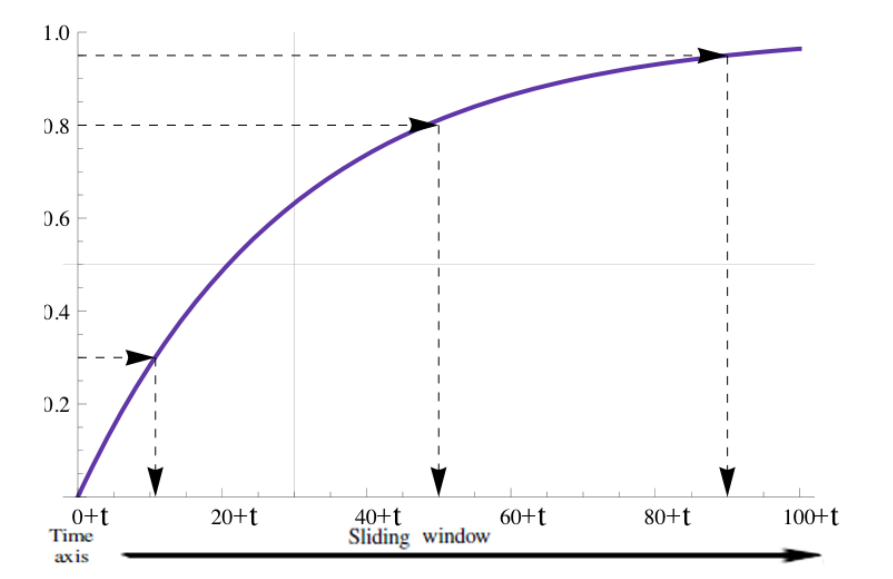
\includegraphics[scale=0.40]{images/choix_exp}
\caption[]{Exemple de distribution exponentielle\footnotemark.
Cela va donc permettre de choisir les points les plus proches avec une probabilité plus grande.}
\end{figure}

\footnotetext{Source: \cite{descente_du_gradient_stochastique}}

\paragraph{}
L'autre point important est le \textit{warm start}. C'est une pré-optimisation.
Il s'agît d'initialiser les paramètres du gradient d'une certaine manière afin d'augmenter la vitesse et les chances
de convergence. Pour ce faire, la meilleure option trouvée dans l'article \cite{descente_du_gradient_stochastique}
consiste à utiliser les valeurs obtenues lors de la précédente itération.
Par conséquent, l'algorithme convergera plus vite pour un coût plus faible en termes d'erreur de calcul.

\paragraph{}
La métrique d'évaluation est différente des notions de \textit{TPR},\textit{TNR} et \textit{TR}.
Dans cet article, le but est de prédire le prix d'un cours, comme EUR/USD à partir de plusieurs autres,
comme EUR/CAD, EUR/AUD, EUR/GBP. Il est donc extrêmement compliqué de calculer avec plusieurs décimales
le résultat exacte, impliquant donc des taux nuls pour chacune des métriques.
Il fallu donc trouver une méthode basée sur l'erreur relative :
$$relative_{error} = \frac{\Delta x}{x}$$

Cela quantifie la différence entre le résultat calculé et le résultat réel tout en le pondérant.

\subsubsubsection{Résultats}
\paragraph{}
Le but est de calculer un taux de change à partir de données. Pour obtenir ces résultats précis, l'auteur a pris le
\textit{Singapore Hedge Fund FOREX Data Set} ainsi que le \textit{Capital K FOREX Data Set}. Les dates ainsi que la fréquence
ne sont pas précisées dans l'article.

L'algorithme retourne deux valeurs : le \textit{bid} et le \textit{ask} à partir des données fournies. Ci-dessous, nous allons
voir la précision de ces résultats. Les tableaux représentent la
comparaison entre les valeurs calculées et les valeurs réelles, soit l'erreur relative.

\begin{table}[H]
	\centering
\begin{tabular}{|l|l|l|l|}
	\hline
	Données & \textit{plainSGD} & \textit{approxSGD} & \textit{approxWarmSGD}\\
	\hline
	\ & \textit{Bid/Ask} & \textit{Bid/Ask} & \textit{Bid/Ask} \\
	\hline
	\textit{Singapoore with SW-1\footnotemark{}} & 0.1366274551\% & 0.133887583\% & 0.2294997927\% \\
	\hline
	\textit{Singapoore with SW/2\footnotemark{}} & 0.1366274551\% & 0.09281447603\% & 0.1551851906\%\\
	\hline

\end{tabular}
\caption[]{Tableau de résultats\footnote[3]{} pour les différentes versions de \textit{SGD} sur le
\textit{FOREX} de Singapore. Les différences entre le \textit{bid} et le \textit{ask} étant minimes,
l'auteur ne les a pas consignées.}
\end{table}

 \addtocounter{footnote}{-2} %3=n
\stepcounter{footnote}\footnotetext{$SW-1$ signifie une fenêtre de choix de taille $N-1$.}
\stepcounter{footnote}\footnotetext{$SW/2$ signifie une fenêtre de choix de taille $N/2$.}
\stepcounter{footnote}\footnotetext{Source des résultats: \cite{descente_du_gradient_stochastique}.}



\paragraph{}
Les erreurs relatives sont très faibles. Les estimations sont donc très proches des valeurs réelles. De plus, on
remarque que le  changement de la taille de la \textit{SW} peut avoir une grande influence. Sur le \textit{plainSGD}
cela ne change rien, on peut donc en conclure que les $N/2 - 1$ données supplémentaires ne sont pas significatives
dans le calcul. Pour le \textit{approxSGD} et le \textit{approxWarmSGD}, le taux d'erreur diminue. Nous pouvons donc
dire que la fenêtre était trop grande et, pire encore, ajoutait du bruit rendant le calcul moins précis.

D'un point de vue calculatoire c'est très intéressant car il est possible de diminuer la taille de la fenêtre et
donc gagner en vitesse tout en gardant, voir en augmentant, la qualité des résultats.


\begin{table}[H]
	\centering
\begin{tabular}{|l|l|l|l|}
	\hline
	Données & \textit{plainSGD} & \textit{approxSGD} & \textit{approxWarmSGD}\\
	\hline
	\ & \textit{Bid/Ask} & \textit{Bid/Ask} & \textit{Bid/Ask} \\
	\hline
	\textit{Capital K SW-1} & 0.01167\%/0.0117\% & 0.0116\%/0.0117\% & 1.502e-03\%/1.554e-03\% \\
	\hline
	\textit{Capital K SW/2} & 0.01167\%/0.0117\% & 0.0314\%/0.0313\% & 1.701e-03\%/1.751e-03\%\\
	\hline

\end{tabular}
\caption[]{Tableau de résultats\footnote{} pour les différentes versions de \textit{SGD}.}
\end{table}

\footnotetext{Source des résultats: \cite{descente_du_gradient_stochastique}}

\paragraph{}
Nous constatons qu'il n'y a pas de différence pour le \textit{plainSGD} entre les deux tailles de fenêtres. On
remarque cependant que pour les deux autres variantes, la diminution de la taille les pénalise. Cependant, l'ordre
de grandeur des erreurs demeure faible. Il est donc important de savoir si nous voulons un chiffre précis ou obtenir
le résultat de manière rapide. L'objectif aiguillera le choix pour l'une ou l'autre des fenêtres.

À noter, que le \textit{approxWarmSGD} obtient de meilleures valeurs que ces concurrents et subit beaucoup moins
les effets de la diminution de \textit{SW} que le \textit{approxSGD}.

\subsection{Conclusion}
\paragraph{}
Afin d'élaborer des algorithmes de \textit{ML}, il est important de saisir les considérations théoriques.
À partir de ces connaissances, le choix d'un algorithme est plus aisé. En effet, si vous voulez apprendre une fonction
continue, mieux vaut utiliser des techniques de descente de gradient et dans le cas de données faiblement différentiables, 
l'utilisation d'un programme \textit{SVM} avec un \textit{kernel trick} est recommandée.

Cela est également valable pour sa mise en place. Les optimisations mathématiques possibles sont nombreuses et complexes,
comme nous l'avons vu dans la partie (\ref{section machine learning finance}), il conviendra donc de les comprendre afin de
mieux cerner les contraintes et les gains lors de l'optimisation.

Ces éléments peuvent être vus comme une boîte à outils algorithmiques, le choix et l'utilisation des différents
outils reviendra à la personne qui programmera. Ce sera cette dernière qui devra construire l'algorithme le plus
adapté avec les données, les contraintes et les techniques à sa disposition.

\paragraph{}
Les considérations mathématiques ne sont pas les seuls éléments importants. Appliquer un algorithme sans chercher à comprendre
les cas concrets peut mener à des programmes peu efficaces.

Dans chacun des articles, les auteurs avaient une connaissance et une compréhension du monde de la finance suffisante,
pour améliorer les techniques en dehors du carde mathématique. L'approche par secteur \cite{machine_learning_automated_trading}
ou l'utilisation de méta-paramètres propre au domaine financier ~\cite{fx_trading} en sont des exemples concrets.
Chacun de ces éléments a sensiblement amélioré les performances des algorithmes auxquels ils ont été appliqués.

Une technique de \textit{machine learning} n'est qu'une solution à un problème mathématique précis. L'ajout d'éléments,
comme ceux cités auparavant, améliore la quantité d'informations disponible et précise l'équation mathématique à optimiser.

\paragraph{}
Il est important de lier ces deux parties pour obtenir des résultats optimaux.

Les valeurs peuvent être encourageantes même s'il convient de relativiser les résultats. Ces derniers ayant pu
être obtenus sur des ensembles de données "faciles". Ce mot qualifie des périodes avec peu de changements ou peu de
variations, ce qui facilite grandement la classification.
Néanmoins, les taux d'erreurs sont faibles et la classification efficace.
Cela démontre que les bons algorithmes appliqués avec une bonne connaissance du domaine fournissent des résultats satisfaisants. 

\paragraph{}
Le choix d'implémenter l'algorithme de réseau de neurones provient des justifications suivantes :
\begin{itemize}
 \item Les \textit{Neural Nets} peuvent, avec assez de ressources\footnote{Cela comprend le temps et les données.}, approximer n'importe
 quel fonction. De plus ils sont capables d'opérer des séparations non linéaires sans recourir au \textit{Kernel trick}.
 \item Il est possible d'éviter les problèmes de sur-apprentissage, en modifiant les méta-paramètres. Cela nous permet de profiter
 de n'importe quel ensemble d'entraînement sans craindre que ce dernier pose problème.
\end{itemize}

Les algorithmes d'arbres de décision sont des classifieurs linéaires. Ce qui signifie qu'ils sont limités
lorsque les données ne sont pas linéaires, réduisant de fait, la qualité de classification. On retrouve ce même problème
pour la régression logistique. De plus les arbres de décision (voir \ref{section arbre de décision}) ont de gros risques
de sur-apprentissage même avec un ensemble d'entraînement adapté, sans compter qu'ils gèrent mal les exemples en continues.
En effet, lors d'un entraînement \textit{online}\footnote{Quand les exemples arrivent de manière continue.} chacun des nouveaux
éléments peut introduire des exceptions. Ce qui implique de reconstruire l'arbre, ce cas pouvant être très lourd en termes
de calculs, il convient donc de l'éviter.

Le classifieur \textit{Naive Bayes} aurait pu être une solution car ce dernier peut classifier les données non linéaires,
ne présente pas de problème de sur-apprentissage et est adapté pour un apprentissage \textit{online}. Il suffit de rajouter le
dernier exemple dans l'équation pour mettre à jour l'apprentissage. La raison qui nous a poussé à choisir les réseaux de neurones 
plutôt que l'algorithme de \textit{Naive Bayes} est que ce dernier a des performances limitées sur un grand ensemble de données.
Si l'on prend des petits jeux de données, \textit{Naive Bayes} est très efficace
\footnote{Dans ce cadre précis, il est même meilleur que tous les autres algorithmes vus dans ce projet.}
\cite{ml_petites_donnees}.
Cependant si l'ensemble grandit, ces performances plafonnent, ce qui n'est pas le cas du \textit{Neural Nets} dont les
résultats augmentent à mesure que le nombre de données disponibles croît.

Au vu des raisons susmentionnées, un algorithme de réseau de neurones nous semblait le meilleur choix, car le \textit{FOREX} nous
fournit suffisamment de données pour avoir d'excellent résultats, de plus, nous ne sommes pas limités par une classification linéaire.


\newpage
%%%%%%%%%%%%%%%%%%%%%%%%%%%%%%%%%%%%%%%%%%%%%%%%%%%%%%%%%%%%%%%%%%%%%%%%%%
% début du projet  %%%%%%%%%%%%%%%%%%%%%%%%%%%%%%%%%%%%%%%%%%%%%%%%%%%%%%%
%%%%%%%%%%%%%%%%%%%%%%%%%%%%%%%%%%%%%%%%%%%%%%%%%%%%%%%%%%%%%%%%%%%%%%%%%%
\section{Projet}
\newpage

%%%%%%%%%%%%%%%%%%%%%%%%%%%%%%%%%%%%%%%%%%%%%%%%%%%%%%%%%%%%%%%%%%%%%%%%%%
% début de la bibliographie %%%%%%%%%%%%%%%%%%%%%%%%%%%%%%%%%%%%%%%%%%%%%%
%%%%%%%%%%%%%%%%%%%%%%%%%%%%%%%%%%%%%%%%%%%%%%%%%%%%%%%%%%%%%%%%%%%%%%%%%%

\bibliographystyle{plain}
\nocite{*}
\bibliography{bibliographie}


\end{document}